\section{问题二模型的建立与求解}
\label{sec:problem2}

\subsection{问题分析与建模思路}

问题二在经典参数--数据标度律上引入数据质量，并检验问题一的领域配比规律能否迁移到附件 B 的绝对 Loss 尺度。决策变量包括模型参数量 $N$、训练 Token 数 $D$、质量水平 $Q_A\in[0,1]$ 和 $17$ 域配比 $\boldsymbol p$；本问输出验证集交叉熵损失模型，供问题三在算力约束下调用。

附件 A 与附件 B 的实验对象和响应尺度不同，不能直接联合回归。本文先由 B1 识别经典标度律，再由 B7 估计质量惩罚，并将问题一的质量向量、参考配比和归一化配比响应作为冻结输入。模型分为固定参考配比的主接口 $\widehat L_{\mathrm{main}}(N,D,Q_A\mid\boldsymbol p_{\mathrm{ref}})$ 与带配比迁移项的情景扩展；前者用于资源分析，后者仅在强度可识别且不违反不可约损失下界时才允许进入决策。

求解依次完成基础模型选择、质量修正选择、资源弹性与等价关系计算以及配比接口验收，并以留出误差、排序保持、bootstrap 稳定性和物理下界作为共同门槛。

\begin{center}
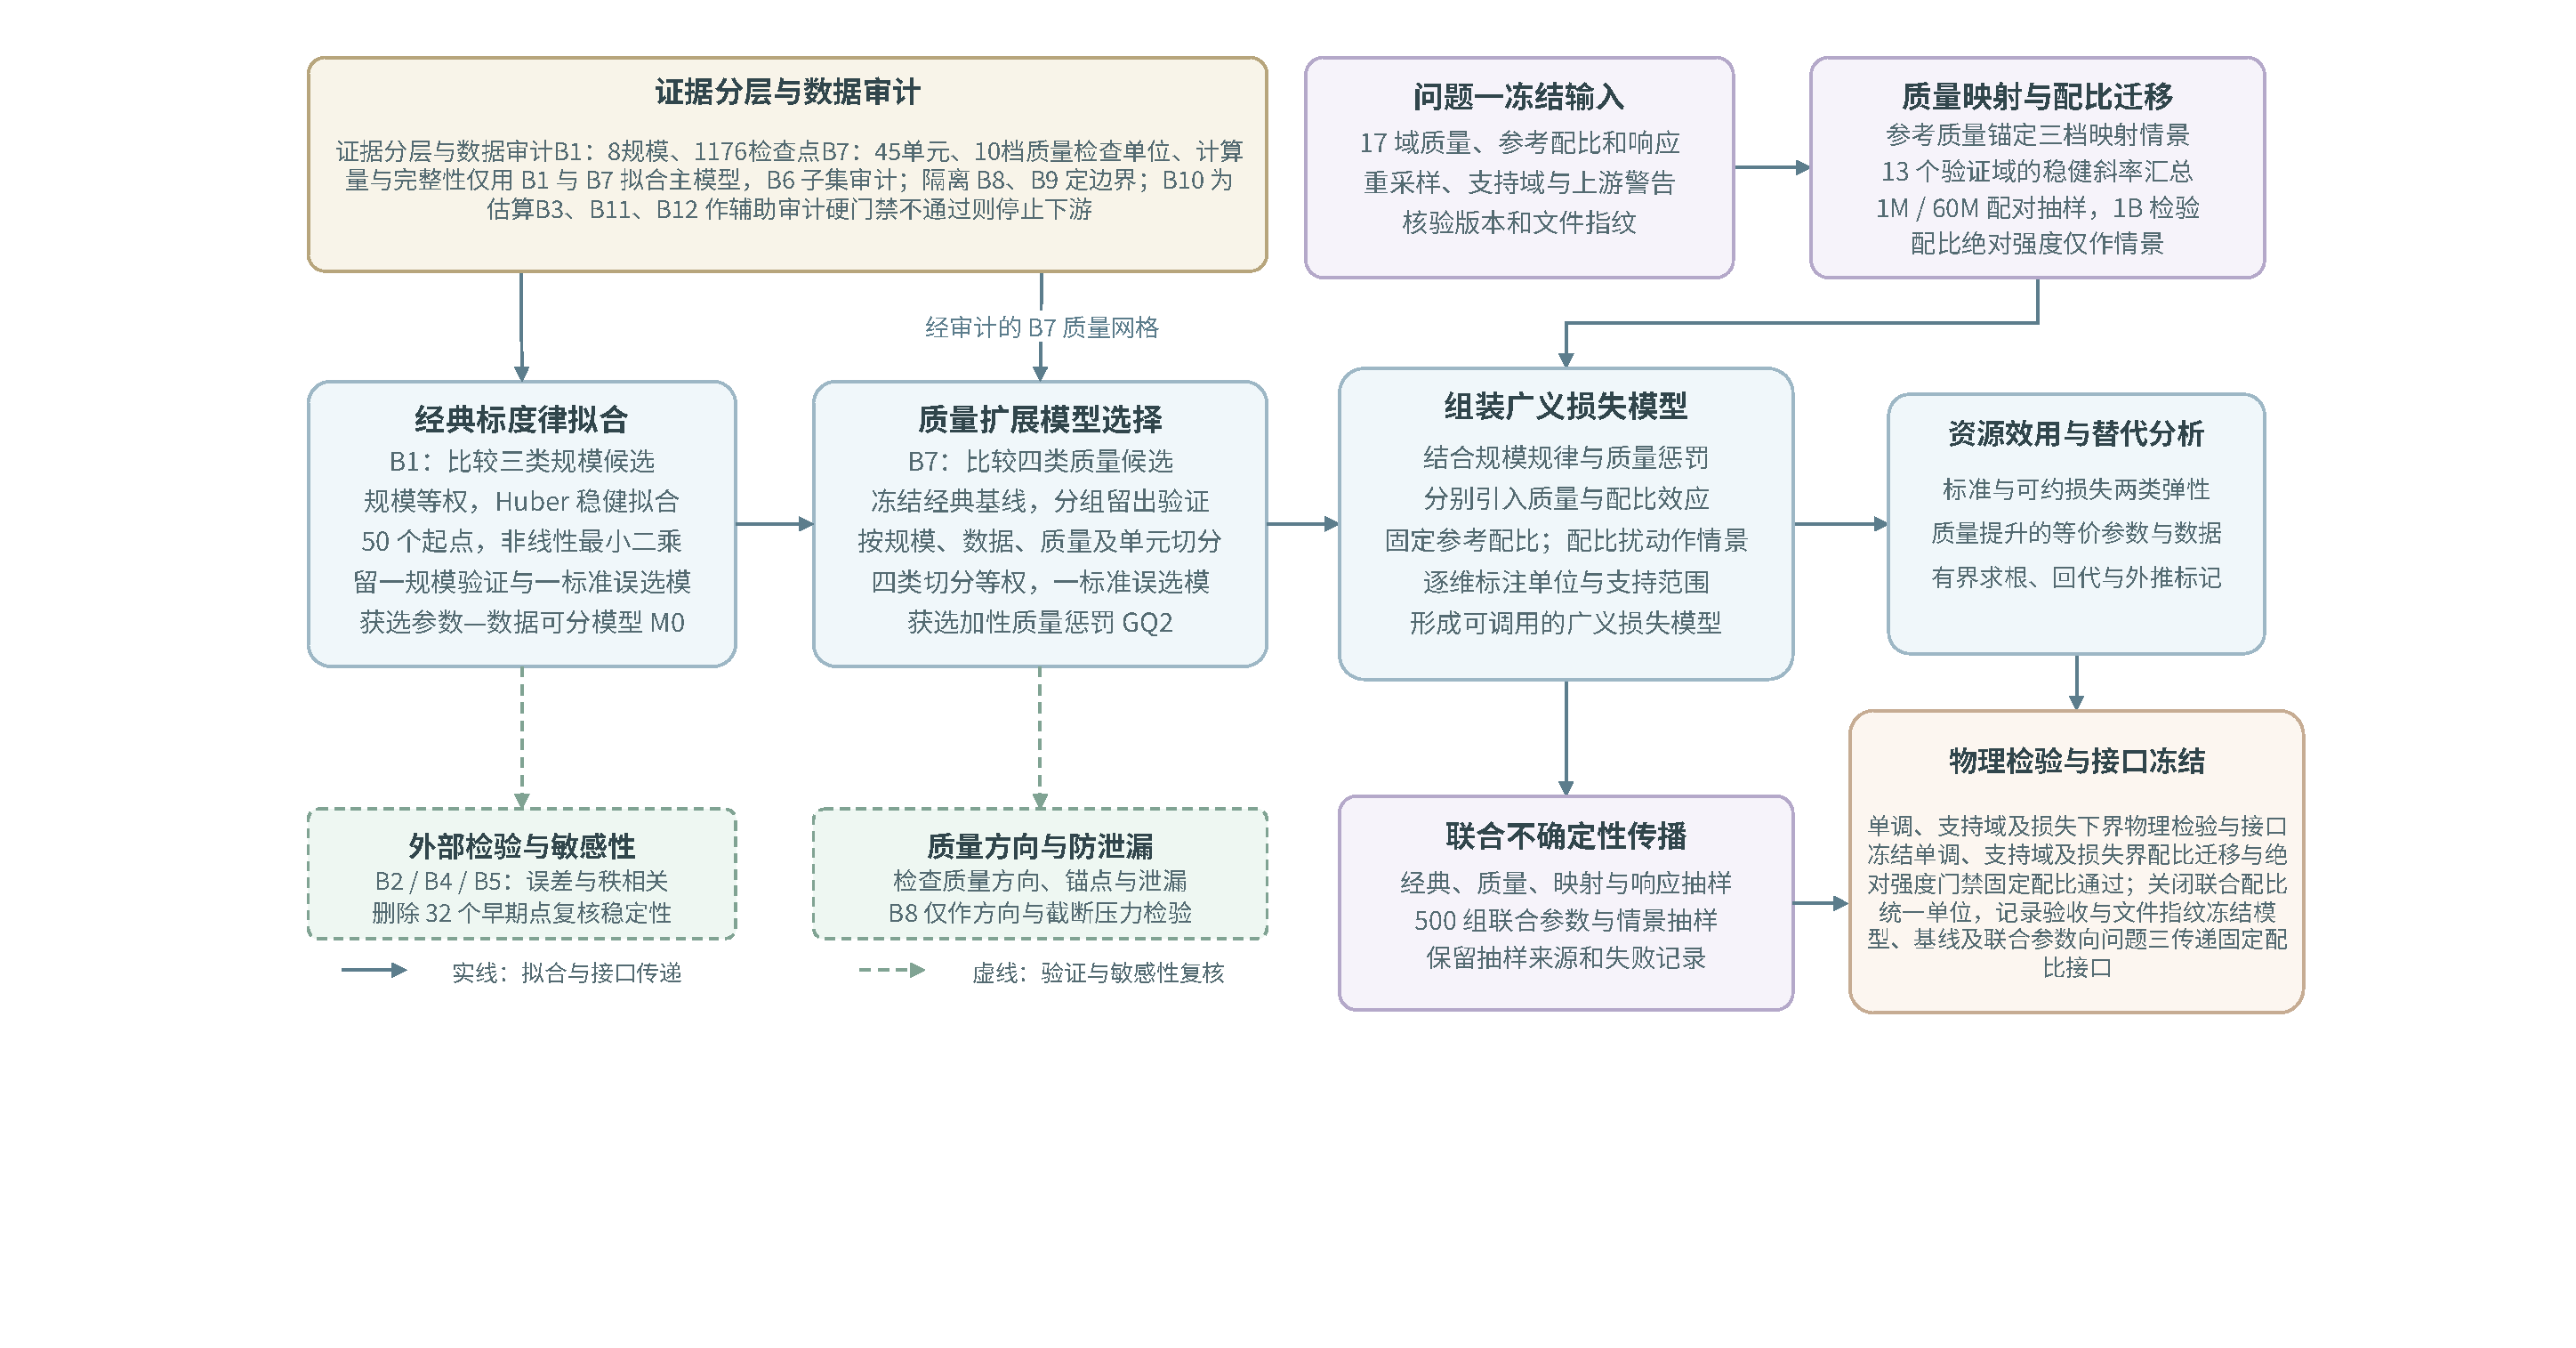
\includegraphics[width=0.96\linewidth]{images/no2/P2_F00_问题二求解流程图.pdf}
\captionof{figure}{问题二广义标度律的构建、检验与接口验收流程}
\label{fig:p2_solution_flow}
\end{center}

图~\ref{fig:p2_solution_flow} 以实线串联证据审计、模型拟合、资源分析与接口冻结，以虚线标出外部验证和敏感性复核；仅通过物理下界与稳定性门槛的接口才传入问题三。

\subsection{输入、数据与证据边界}

\subsubsection{数据审计与证据分层}

附件 B 的数据来源与可信程度不同，本文不作整表混合，而按表~\ref{tab:p2_evidence} 分配拟合、验证、压力测试和外推角色。参数量和训练数据量统一写为十亿尺度 $n=N/10^9$、$d=D/10^9$。

\begin{table}[!htbp]
\centering
\small
\setlength{\tabcolsep}{4pt}
\caption{附件 B 的证据分层与使用方式}
\label{tab:p2_evidence}
\begin{tabular}{p{0.13\linewidth}p{0.33\linewidth}p{0.43\linewidth}}
\toprule
数据源 & 数据性质 & 本问用途 \\
\midrule
B1 & $1176$ 条真实轨迹，覆盖 $8$ 个规模 & 拟合经典标度律并执行留一规模验证 \\
B2--B5 & 半合成轨迹、同源插值、跨族记录与文献数据 & 冻结参数后的外部一致性和排序检验 \\
B6--B7 & 分块质量实验，B6 为 B7 子集 & B6 作一致性核对，B7 的 $45\times10$ 网格拟合质量项 \\
B8 & 扩展质量网格，含反向响应和截断记录 & 仅作方向冲突与边界压力测试 \\
B9--B10 & 大模型规模信息与估算 Loss & 标记外推范围和量级，不增加独立观测证据 \\
B11--B12 & 模型族元数据与检查点索引 & 来源确认和轨迹完整性审计 \\
\bottomrule
\end{tabular}
\end{table}

据此记拟合集为 $\mathcal D_{\mathrm{fit}}=\{\mathrm{B1},\mathrm{B7}\}$，外部验证集主要由 B2--B5 构成，B8--B10 仅界定压力测试与外推边界。问题一的质量与配比结果同样以冻结接口输入，避免重复计算和跨体系信息泄漏。

\subsection{模型建立}

\subsubsection{经典参数—数据标度律模型}

以 $n=N/10^9$、$d=D/10^9$ 为无量纲规模，比较参数--数据可分幂律、总计算量幂律和带交互项幂律三类候选模型：
\begin{align}
M_0:\quad L_0(n,d)
&=E+A n^{-\alpha}+B d^{-\beta},
\label{eq:p2_classic_m0}\\
M_C:\quad L_C(n,d)
&=E_C+K_C(6nd)^{-\zeta},
\label{eq:p2_classic_mc}\\
M_{ND}:\quad L_{ND}(n,d)
&=E_{ND}+A_{ND}n^{-\alpha_{ND}}
+B_{ND}d^{-\beta_{ND}}+G(nd)^{-\xi}.
\label{eq:p2_classic_mnd}
\end{align}
其中，$E$ 类参数表示不可约损失，$6nd$ 为训练计算量代理，$G(nd)^{-\xi}$ 用于检验参数量与数据量的额外耦合。所有系数和衰减指数均约束为正，以保证规模增加时预测损失非增。最终依据 B1 的留一规模误差和简约性原则选型，B2--B5 仅用于冻结参数后的外部一致性检验。

\subsubsection{质量与配比的跨体系衔接}

设问题一输出的领域质量向量为 $\boldsymbol q=(q_1,\ldots,q_{17})^{\mathsf T}$，参考配比为 $\boldsymbol p_{\mathrm{ref}}$。任意配比 $\boldsymbol p$ 的加权质量及参考锚点定义为

\begin{equation}
Q_{\mathrm{base}}(\boldsymbol p)
=
\boldsymbol p^{\mathsf T}\boldsymbol q,
\qquad
Q_{\mathrm{ref}}
=
Q_{\mathrm{base}}(\boldsymbol p_{\mathrm{ref}})
=
0.5389559588,
\label{eq:p2_quality_bridge}
\end{equation}

其中 $Q_{\mathrm{base}}$ 是配比加权指标，不是直接观测的训练质量。为避免将问题一的配比 Loss 当作问题二的绝对 Loss，记 $\widehat{\ell}_k^A(\boldsymbol p)$ 为第 $k$ 个验证域的 Scheff\'e--Ridge 预测，$s_k$ 为其四分位距，定义

\begin{equation}
J(\boldsymbol p)
=
\frac{1}{13}
\sum_{k=1}^{13}
\frac{\widehat{\ell}_k^A(\boldsymbol p)}
{s_k},
\label{eq:p2_quality_bridge_J}
\end{equation}

并以参考配比中心化：

\begin{equation}
R(\boldsymbol p)
=
\frac{
J(\boldsymbol p)-J(\boldsymbol p_{\mathrm{ref}})
}
{
\operatorname{IQR}_{A4}[J(\boldsymbol p)]
},
\qquad
R(\boldsymbol p_{\mathrm{ref}})
=
0.
\label{eq:p2_mixture_bridge}
\end{equation}

分母取问题一 A4 样本上 $J(\boldsymbol p)$ 的四分位距，故 $R(\boldsymbol p)$ 只表达相对方向。由于两套质量尺度缺少独立校准实验，采用以 $Q_{\mathrm{ref}}$ 为锚点的情景映射

\begin{equation}
Q_{\mathrm{eff}}:=h_{s_Q}(Q_A)
=
\operatorname{clip}
\left[
Q_{\mathrm{ref}}
+
s_Q(Q_A-Q_{\mathrm{ref}}),
\varepsilon,
1
\right],
\qquad
s_Q\in\{0.5,1,1.5\},
\label{eq:p2_quality_map}
\end{equation}

其中 $s_Q=1$ 为主情景，$s_Q=0.5,1.5$ 用于敏感性分析，$\operatorname{clip}$ 保证有效质量落在可行区间。该映射和 $R(\boldsymbol p)$ 均为跨体系情景接口，不构成质量与配比已获联合实验识别的证据；主模型因此固定 $\boldsymbol p=\boldsymbol p_{\mathrm{ref}}$。

\subsubsection{固定配比主模型与配比迁移扩展}

记 B7 识别的质量惩罚为 $\Delta_Q(n,d,Q_{\mathrm{eff}})$。固定 $\boldsymbol p=\boldsymbol p_{\mathrm{ref}}$ 时，传给问题三的主模型为
\begin{equation}
\widehat L_{\mathrm{main}}(N,D,Q_A)
=L_0(n,d)+\Delta_Q\!\left(n,d,Q_{\mathrm{eff}}\right),
\qquad Q_{\mathrm{eff}}=h_{s_Q}(Q_A).
\label{eq:p2_main_interface}
\end{equation}
为检验问题一的相对配比响应能否进入 B 体系，再引入尺度迁移系数 $\lambda_0$ 和规模调整项 $(n/n_0)^{\delta_p}$，其中 $n_0$ 为 B7 参数规模中位数，得到情景扩展

\begin{equation}
\widehat L(N,D,Q_A,\boldsymbol p)
=
L_0(n,d)
+
\Delta_Q
\left(
n,d,Q_{\mathrm{eff}}
\right)
+
\lambda_0
\left(
\frac n{n_0}
\right)^{\delta_p}
R(\boldsymbol p),
\qquad
n=\frac{N}{10^9},
\quad
d=\frac{D}{10^9}.
\label{eq:p2_generalized}
\end{equation}

其中，$\lambda_0$ 连接 A、B 两套损失尺度，$\delta_p$ 描述配比效应随规模的变化。由于缺少四因素联合实验，非零 $\lambda_0$ 只作预设强度情景，不能视为可识别参数。主接口中 $R(\boldsymbol p_{\mathrm{ref}})=0$；进一步取 $Q_A=1,s_Q=1$ 时 $\Delta_Q=0$，模型恢复为 $L_0(n,d)$。超出 B 系列支持域的结果仅解释趋势，并保留外推标记。

\subsubsection{边际效用与资源等价指标构建}

令 $x\in\{N,D,Q_A\}$。局部边际效用取 $u_x=-\partial\widehat L/\partial x$；为消除资源量纲差异，进一步定义总损失弹性与可约损失弹性：

\begin{equation}
\epsilon_x=-\frac{x}{\widehat L}\frac{\partial\widehat L}{\partial x},
\qquad
\epsilon_x^{\mathrm{red}}=-\frac{x}{\widehat L-E}\frac{\partial\widehat L}{\partial x}
\quad(\widehat L>E).
\label{eq:p2_elasticity}
\end{equation}

前者衡量整体 Loss 的相对变化，后者以剩余可降低部分归一化，二者不混用。在固定参考配比且 $\lambda_0=0$ 的主情景下，GQ2 质量项为 $\Delta_Q=c_Q[1-h_{s_Q}(Q_A)]^{\nu_Q}$；映射未触及截断边界时，有

\begin{equation}
\frac{\partial\widehat L}{\partial N}
=
-\frac{\alpha A n^{-\alpha}}{N},
\qquad
\frac{\partial\widehat L}{\partial D}
=
-\frac{\beta B d^{-\beta}}{D},
\qquad
\frac{\partial\widehat L}{\partial Q_A}
=
-c_Q\nu_Q
[1-h_{s_Q}(Q_A)]^{\nu_Q-1}s_Q .
\label{eq:p2_derivatives}
\end{equation}

在等损失条件 $\mathrm d\widehat L=0$ 下，一阶 Taylor 展开给出质量提升的局部资源等价关系：

\begin{equation}
\Delta\log N
\simeq
\frac{
\partial\widehat L/\partial Q_A
}
{
N\,\partial\widehat L/\partial N
}
\Delta Q_A,
\qquad
\Delta\log D
\simeq
\frac{
\partial\widehat L/\partial Q_A
}
{
D\,\partial\widehat L/\partial D
}
\Delta Q_A.
\label{eq:p2_local_equivalence}
\end{equation}

对于较大质量变化，改用有限变化方程
\begin{align}
\widehat L(N',D,Q_A,\boldsymbol p_{\mathrm{ref}})
&=\widehat L(N,D,Q_A+\Delta Q_A,\boldsymbol p_{\mathrm{ref}}),\nonumber\\
\widehat L(N,D',Q_A,\boldsymbol p_{\mathrm{ref}})
&=\widehat L(N,D,Q_A+\Delta Q_A,\boldsymbol p_{\mathrm{ref}})
\label{eq:p2_finite_equivalence}
\end{align}
分别求得参数等价相对增幅 $r_N=N'/N-1$ 和数据等价相对增幅 $r_D=D'/D-1$。

上述等价量只比较模型预测的 Loss 变化，不表示计算成本、训练时间或经济成本相同。

\subsection{模型求解}

\subsubsection{经典标度律与质量修正模型参数估计}

不同模型层的数据来源和证据强度不同，故采用分阶段估计而不作四因素联合拟合。B1 拟合中以模型规模为聚类单位赋予等权重，使用 Huber 稳健非线性最小二乘和对数参数化 $\theta=\exp(\eta)$，并以拉丁超立方多起点降低初值影响。

模型评价按参数规模整体留一；当候选误差接近时，依照 one-SE 原则选择结构更简单者。验证结果见表~\ref{tab:p2_classic_cv}。

\begin{table}[!htbp]
\centering
\caption{经典标度律的留一模型规模验证结果}
\label{tab:p2_classic_cv}
\begin{tabular}{lrr}
\toprule
候选模型 & RMSE & 归一化 RMSE \\
\midrule
$M_0$ & 0.000147 & 0.000374 \\
$M_C$ & 0.084910 & 0.216303 \\
$M_{ND}$ & 0.000148 & 0.000376 \\
\bottomrule
\end{tabular}
\end{table}

实验结果表明，参数—数据可分幂律模型 $M_0$ 的留一规模 RMSE 为 $0.000147$，归一化 RMSE 为 $0.000374$；带交互项模型 $M_{ND}$ 的对应指标分别为 $0.000148$ 和 $0.000376$。虽然 $M_{ND}$ 增加了参数—数据交互项，但其验证误差并未降低，说明在当前 B1 数据范围内，额外交互结构未提供额外预测能力。因此，根据 one-SE 原则，选择结构更简洁的 $M_0$ 作为基础标度律模型。

\begin{figure}[!htbp]
\centering
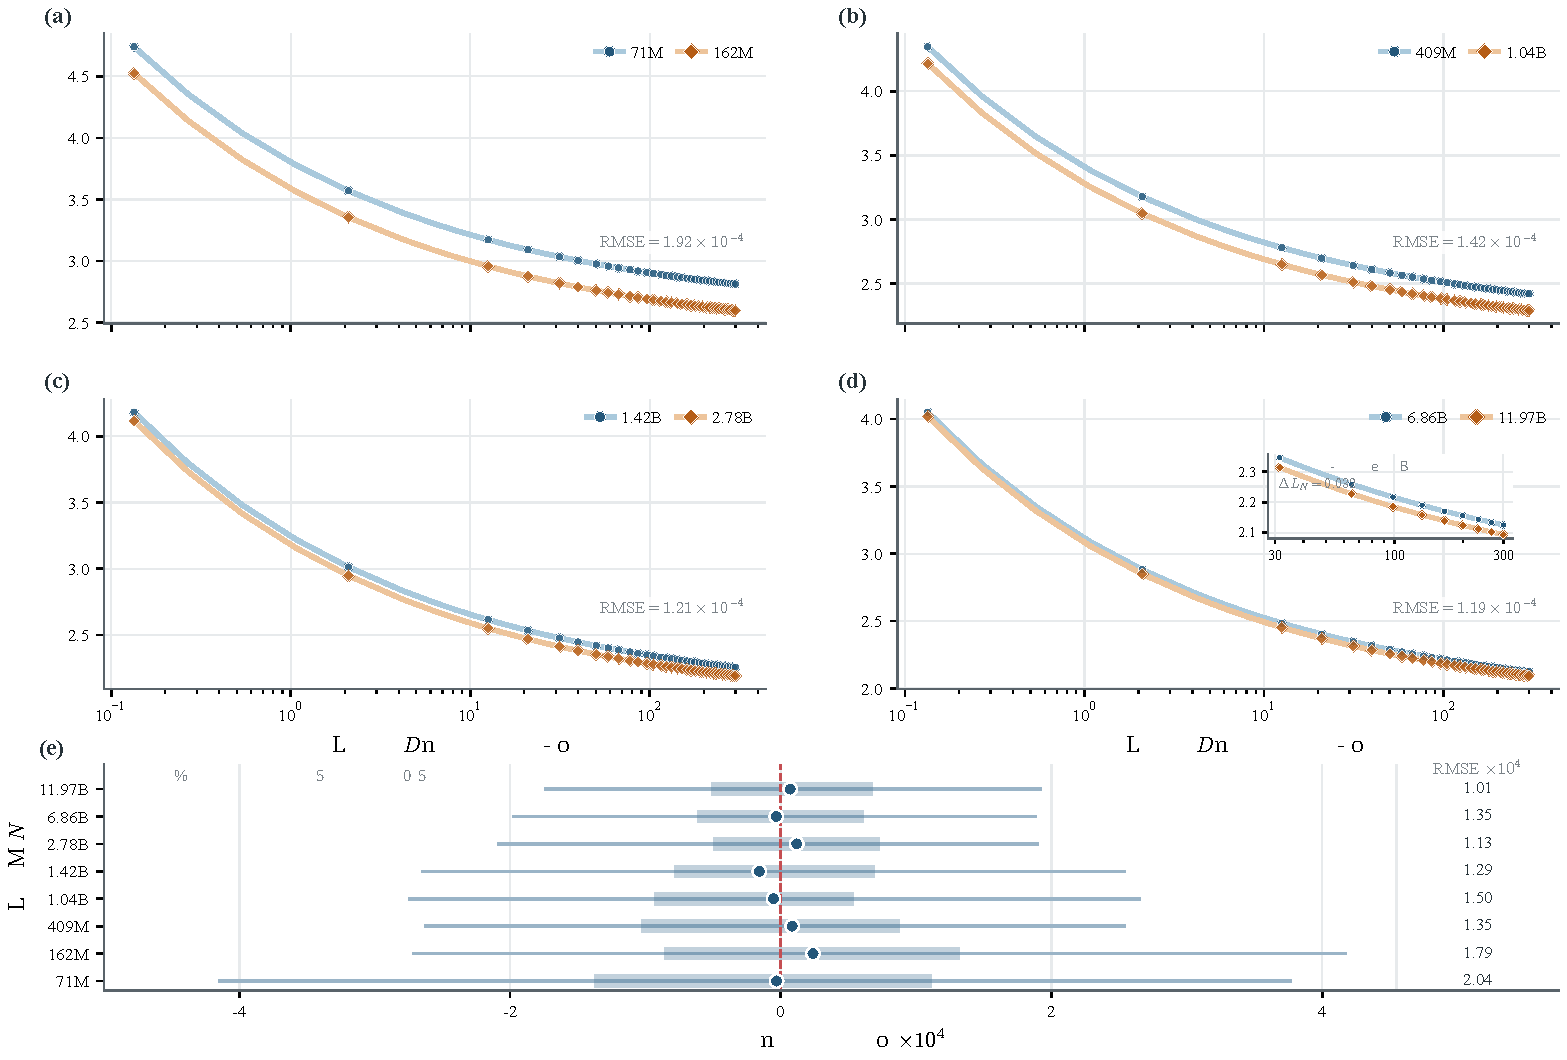
\includegraphics[width=0.98\linewidth]{images/no2/P2R_F01_经典标度律拟合与数据坍缩.pdf}
\caption{经典标度律在八种参数规模下的局部拟合与残差诊断}
\label{fig:p2_classic_fit}
\end{figure}

图~\ref{fig:p2_classic_fit} 将八条 B1 训练轨迹按参数规模两两分组。四个局部子图中，深色散点为观测检查点，浅色曲线为 $M_0$ 拟合结果；底部区间图进一步汇总各规模的残差范围和 RMSE。拟合曲线能够追踪不同模型规模下损失随 Token 增加的衰减趋势，且各规模残差均围绕零值分布，与留一规模验证对 $M_0$ 的选择相一致。

固定 B1 参数后，以 B7 估计增量质量项 $\widehat L=L_0(n,d)+\Delta_Q(n,d,Q)$。验证分别按参数规模、数据规模、质量水平和 $(N,D)$ 单元成块留出，各切分等权；验证折不提供 $Q_B=1$ 基线，以避免信息泄漏。依据成块误差和 one-SE 原则选择 GQ2。

\begin{figure}[!htbp]
\centering
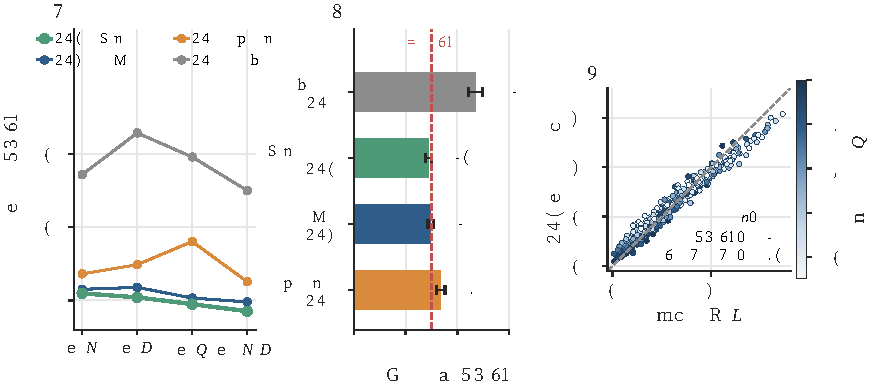
\includegraphics[width=0.98\linewidth]{images/no2/P2R_F02_质量模型成块交叉验证选择.pdf}
\caption{质量响应候选模型的成块交叉验证比较}
\label{fig:p2_quality_model_selection}
\end{figure}

图~\ref{fig:p2_quality_model_selection} 表明，GQ2 在 $69$ 个留出块上的等权 RMSE 为 $0.072$，较 GQ1 降低 $38.7\%$；其留数据规模、参数规模、质量水平和资源单元 RMSE 分别为 $0.073338$、$0.074643$、$0.071086$ 和 $0.068770$，优势并非由单一切分偶然造成。

\begin{center}
\centering
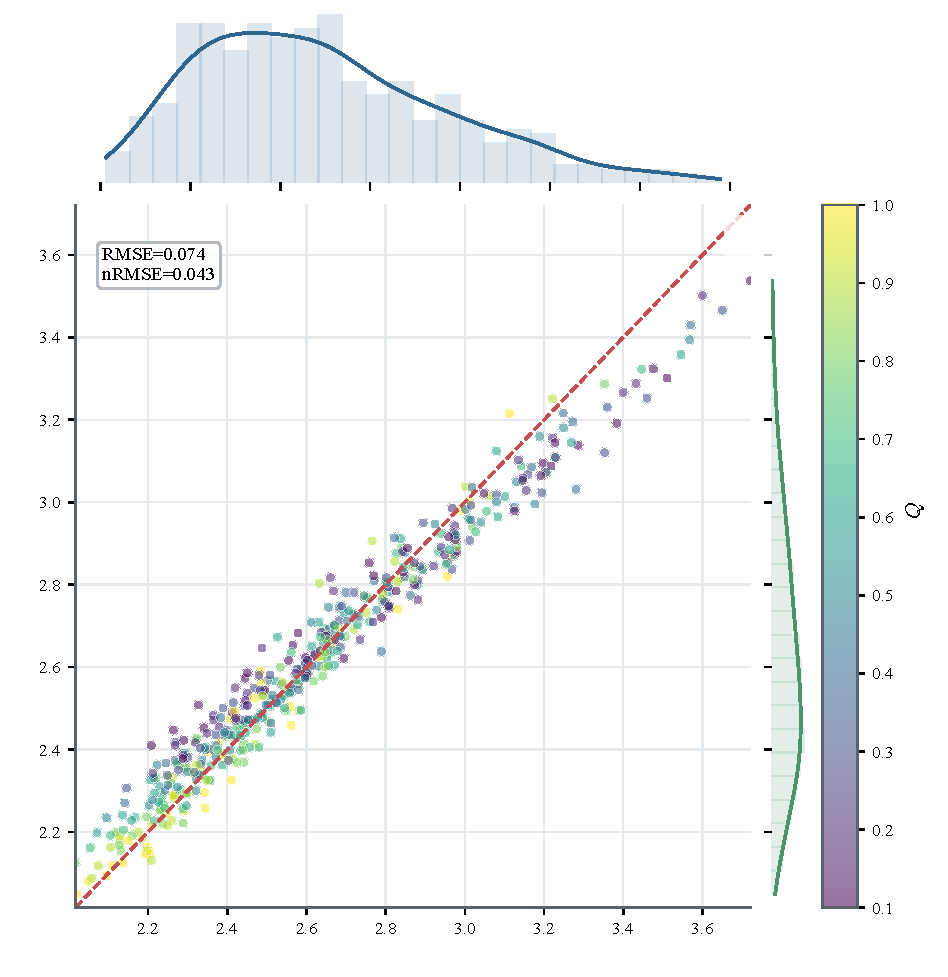
\includegraphics[width=0.74\linewidth]{images/no2/P2R_F03_GQ2预测观测边缘分布.pdf}
\captionof{figure}{GQ2 留资源单元验证的预测值与观测值联合分布}
\label{fig:p2_gq2_joint}
\end{center}

图~\ref{fig:p2_gq2_joint} 展示留 $(N,D)$ 资源单元验证中的逐点预测结果。中心散点按质量水平 $Q$ 着色，上方和右侧分别给出观测 Loss 与预测 Loss 的边缘分布。大部分样本沿 $1{:}1$ 线附近排列，说明模型能够捕捉主要变化趋势；高 Loss 尾部仍存在一定低估，因此后续外推仍需与支持域和压力测试结果结合解释。

随后，以 $(N,D)$ 资源单元作为 bootstrap 重采样簇，对质量修正参数进行 $500$ 次重复抽样，获得参数稳定性范围。在参考质量 $Q_{\mathrm{ref}}=0.538956$ 处，质量提高 $0.05$ 时预测 Loss 降低 $0.018071$，bootstrap $95\%$ 区间为 $[0.016565,\,0.019604]$；质量提高 $0.10$ 时预测 Loss 降低 $0.036164$，对应区间为 $[0.033208,\,0.039190]$。两组区间均未跨越零，说明当前实验支持域内的提质收益方向稳定。

问题一的配比信息不作为直接拟合参数，而通过冻结质量映射、Scheff\'e 响应和迁移抽样传播至广义模型。对 $1\mathrm{M}$、$60\mathrm{M}$ 和 $1\mathrm{B}$ 检验集，以稳健回归检验 $R(\boldsymbol p)$ 与标准化 Loss 的方向，并由前两个尺度的斜率比估计 $\delta_p$；因 A、B 体系缺少联合观测，非零配比强度只作预设情景。

最终得到基础标度律和质量修正参数估计结果：

\begin{equation}
\begin{aligned}
&(E,A,B,\alpha,\beta)
=
(1.6898,\,
0.35398,\,
1.24031,\,
0.339977,\,
0.279878),\\
&(c_Q,\nu_Q)
=
(0.36204,\,
0.990288).
\end{aligned}
\label{eq:p2_estimates}
\end{equation}

在 B7 数据的质量锚点 $Q_B=1$ 情景下，模型归一化 RMSE 为 $0.113203$。

B1 与 B7 分别估计经典项和质量项；B8--B10 不参与主模型选择，只承担压力测试和外推边界评估。

\begin{center}
\centering
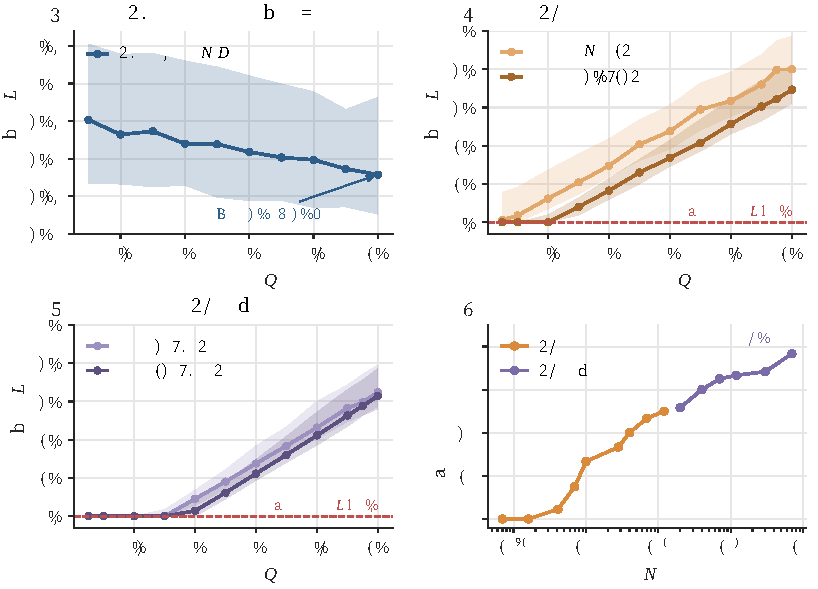
\includegraphics[width=0.99\linewidth]{images/no2/P2R_F04_B7与B8质量响应压力测试.pdf}
\captionof{figure}{B7 主质量网格与 B8 分规模压力测试}
\label{fig:p2_quality_stress}
\end{center}

图~\ref{fig:p2_quality_stress} 对上述证据分层给出直观检查。B7 主网格中 Loss 随质量提高而降低，方向与 GQ2 一致；B8 在部分大规模和远端区域出现方向反转及截断地板。地板记录比例随参数规模增大至 $38.3\%$，表明异常区域不宜反向影响主模型选择，而应作为外推边界和模型风险的压力测试证据。

\subsection{结果分析与模型验证}

\subsubsection{主模型响应与配比迁移方向}

在主身份映射情景 $s_Q=1$、$\boldsymbol p=\boldsymbol p_{\mathrm{ref}}$ 下，有 $Q_{\mathrm{eff}}=Q_A$ 且 $R(\boldsymbol p_{\mathrm{ref}})=0$，配比迁移项不参与主模型预测。因此，冻结标度律仅包含参数规模、训练数据规模和质量修正项：

\begin{equation}
\widehat L
=
1.689798
+
0.353980n^{-0.339977}
+
1.240306d^{-0.279878}
+
0.362040(1-Q)^{0.990288}.
\label{eq:p2_final_fixed_p}
\end{equation}

式~\eqref{eq:p2_final_fixed_p} 中，$E=1.689798$ 表示不可约损失水平。参数项 $0.353980n^{-0.339977}$ 与数据项 $1.240306d^{-0.279878}$ 分别描述两类规模扩张带来的损失下降；质量项 $0.362040(1-Q)^{0.990288}$ 表示训练数据质量偏离高质量状态时产生的额外损失。上述系数和指数均是当前实验支持域内的统计响应参数，而非跨所有模型族与训练策略均保持不变的物理常数。

在领域配比分析方面，问题一的归一化响应 $R(\boldsymbol p)$ 在 $1\mathrm{M}$、$60\mathrm{M}$ 与 $1\mathrm{B}$ 检验尺度下，与综合 Loss 的 Spearman 相关系数分别为 $0.812811$、$0.819749$ 和 $0.734158$。该结果说明配比响应在不同规模下保持一定方向一致性，但由于较大规模数据缺少 A、B 两体系之间的绝对 Loss 对齐信息，本文仅保留方向敏感性，不进行精确强度校准。

\begin{figure}[!htbp]
\centering
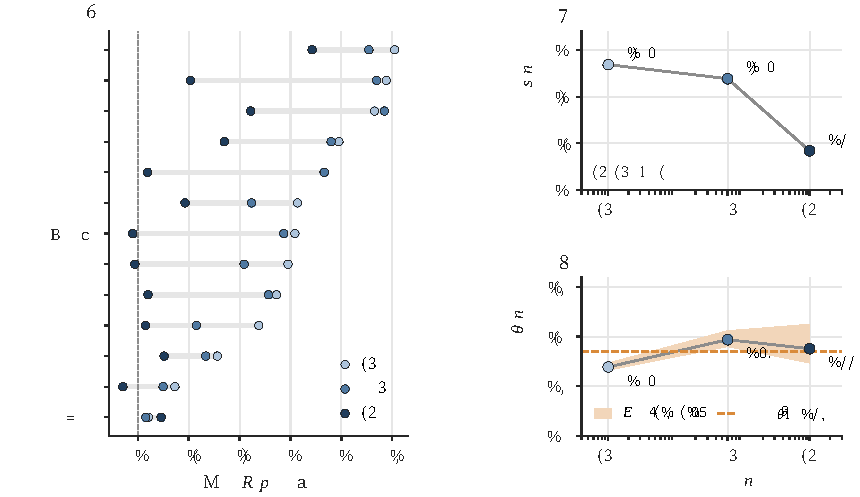
\includegraphics[width=0.96\linewidth]{images/no2/P2R_F05_配比效应跨尺度迁移.pdf}
\caption{配比响应的跨尺度迁移及其不确定性}
\label{fig:p2_mixture_transfer}
\end{figure}

图~\ref{fig:p2_mixture_transfer} 将各领域在三种检验尺度下的配比响应并置比较。$1\mathrm{M}$ 与 $60\mathrm{M}$ 下多数领域保持相同变化方向，而 $1\mathrm{B}$ 的综合响应仅为 $1\mathrm{M}$ 的 $31.2\%$，部分领域的 bootstrap 区间还出现跨零或方向反转。因此，配比结果可以支持跨尺度方向分析，却不足以支持固定强度的跨体系迁移。

进一步分析问题一 Scheff\'e 交互项，bootstrap 分类得到 $75$ 组互补关系和 $61$ 组不确定关系。负向二阶交互项表示相对于简单线性叠加，两个领域组合可能产生额外损失下降，而不确定关系不能解释为已验证的替代效应。候选方案 $\boldsymbol p^\star$ 的归一化响应为 $-2.289763$，bootstrap $95\%$ 区间为 $[-3.568433,\ 0.113031]$；由于该区间包含零，其仅作为敏感性情景，不视为稳定优于参考配比的决策结果。

\subsubsection{广义标度律地形与外推边界}

由式~\eqref{eq:p2_final_fixed_p} 可见，参数规模、数据规模与质量因素均通过衰减项影响预测损失，但其局部作用大小取决于当前资源状态。为同时观察规模效应、质量效应与外推边界，将连续预测曲面及其等 Loss 前沿绘于图~\ref{fig:p2_landscape}。

\begin{figure}[!htbp]
\centering
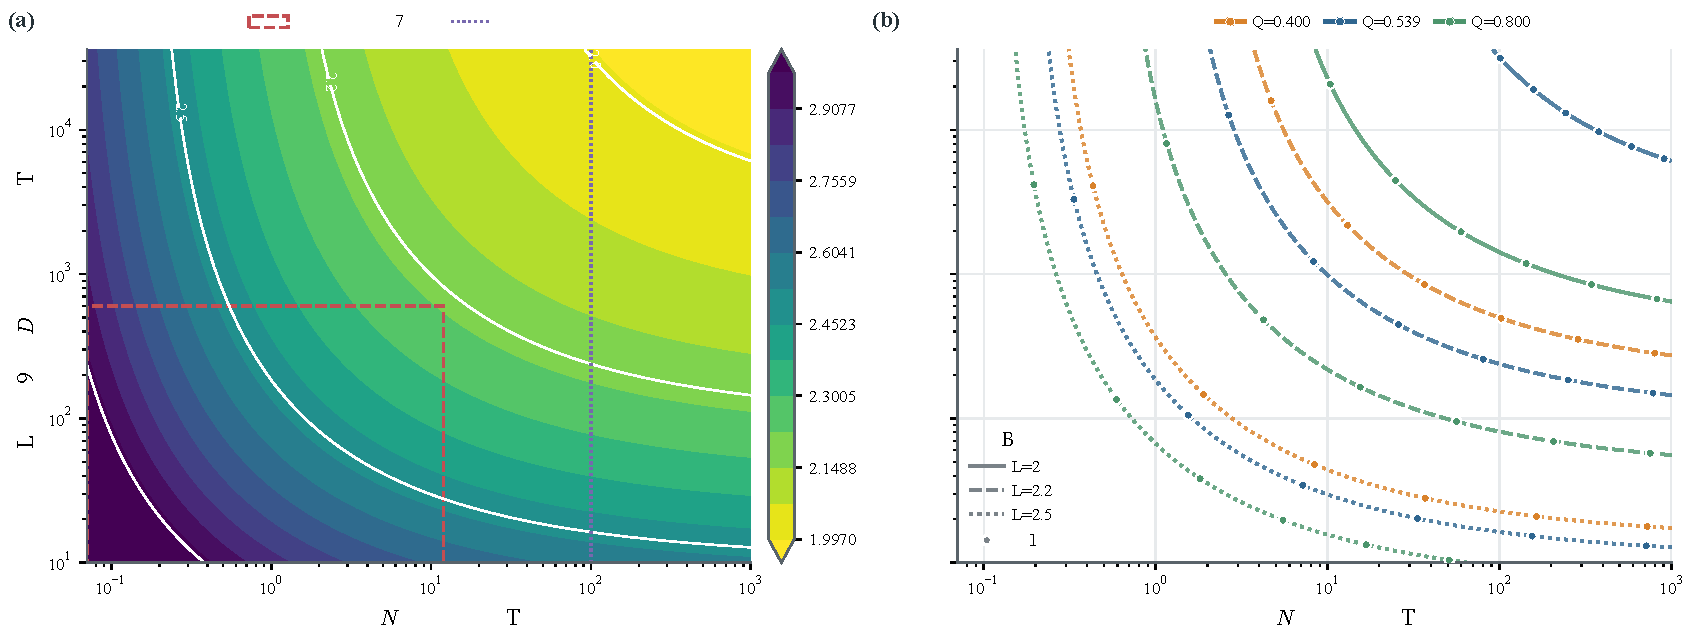
\includegraphics[width=0.98\linewidth]{images/no2/P2R_F06_广义标度律地形与等损失前沿.pdf}
\caption{固定参考配比下的广义标度律地形与等 Loss 前沿}
\label{fig:p2_landscape}
\end{figure}

图~\ref{fig:p2_landscape}(a) 标出 B1/B7 观测支持域与 B9 扩展起点，表明大规模结果在几何上已离开主拟合区域；图~\ref{fig:p2_landscape}(b) 显示，质量提高会使等 Loss 前沿系统向更低的参数量或 Token 量方向移动。图中圆点是从连续模型前沿上抽取的计算节点，而非新的原始观测，因此前沿仅用于资源关系解释，不能被误读为外推区域已获得实验验证。

\subsubsection{资源弹性与有限等价关系}

为比较不同资源在模型所处状态变化时的相对作用，首先计算参数、Token 和质量的标准总 Loss 弹性，并在 $27$ 个 $N$--$D$--$Q$ 网格状态上汇总其组成。

\begin{figure}[!htbp]
\centering
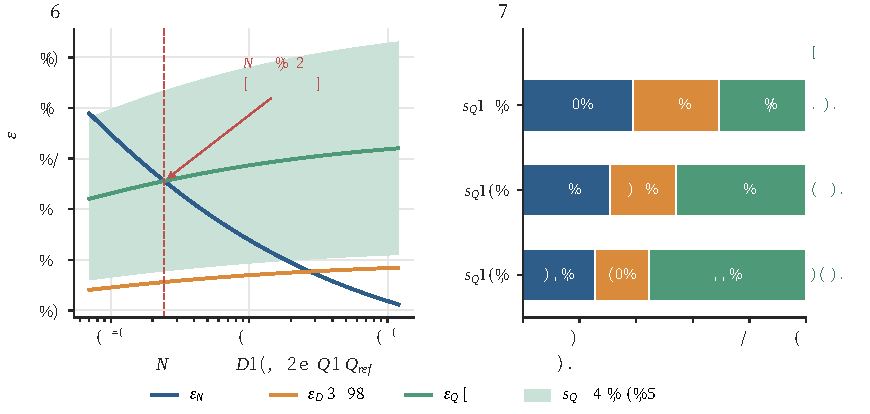
\includegraphics[width=0.96\linewidth]{images/no2/P2R_F07_资源弹性组成状态图.pdf}
\caption{固定参考配比下的资源弹性路径与主导结构迁移}
\label{fig:p2_elasticity}
\end{figure}

图~\ref{fig:p2_elasticity}(a) 在 $D=150\mathrm{B}$ 和参考质量下跟踪三类弹性随参数规模的连续变化；主情景中，质量弹性约在 $N=0.24\mathrm{B}$ 后超过参数弹性。图~\ref{fig:p2_elasticity}(b) 表明，当 $s_Q$ 从 $0.5$ 增加至 $1.5$ 时，质量平均弹性份额由 $30.8\%$ 增至 $55.5\%$，质量主导状态也由 $7/27$ 增至 $21/27$。因此，质量映射强度是资源主导结构的关键不确定性来源。

进一步以 B7 参数规模和数据规模的中位参考点为基准，取 $Q_A=0.538956$、$s_Q=1$、$\Delta Q_A=0.1$，代入式~\eqref{eq:p2_finite_equivalence} 求得资源等价关系。质量评分提高 $0.1$ 时，其损失下降效果分别等价于在原质量水平下将参数规模增加 $r_N=0.372985$，或将训练数据规模增加 $r_D=0.569474$，即约相当于参数扩张 $37.30\%$ 或数据扩张 $56.95\%$。

\begin{figure}[!htbp]
\centering
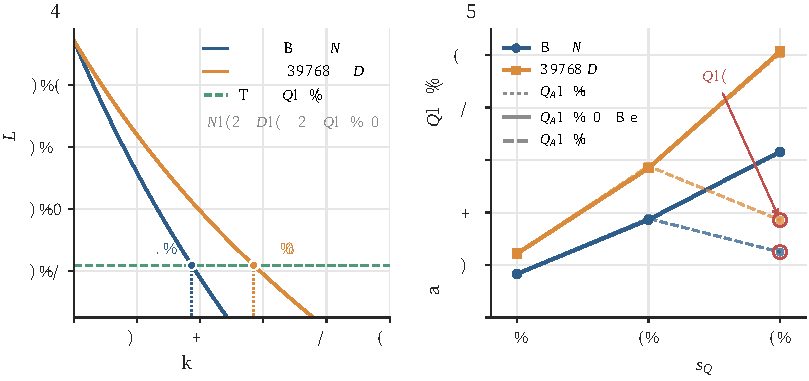
\includegraphics[width=0.95\linewidth]{images/no2/P2R_F08_质量提升的有限资源等价量.pdf}
\caption{质量提升 $0.10$ 的有限资源等价量及其情景变化}
\label{fig:p2_finite_equivalence}
\end{figure}

图~\ref{fig:p2_finite_equivalence}(a) 通过同一目标 Loss 下的两组交点直观展示 $37.30\%$ 和 $56.95\%$ 的有限等价增幅；图~\ref{fig:p2_finite_equivalence}(b) 利用 $18$ 个实际计算点展示结果随基线质量和 $s_Q$ 的变化。高质量且 $s_Q=1.5$ 时，质量映射触及 $Q=1$ 截断边界，因此等价增幅出现回落。该结果只表示模型空间中的性能等价，未计入提升数据质量的实际成本，不能直接解释为工程成本等价。

除标准总 Loss 弹性外，在 $\widehat L>E$ 条件下还可计算可约损失弹性，用于分析距离不可约极限较远区域的资源敏感性。两类弹性的归一化对象不同，不宜直接混用；同时，不同 $s_Q$ 会显著改变等价结果，故跨体系质量映射假设是解释结果的重要前提。

\subsection{敏感性、适用边界与本问输出}

\subsubsection{配比接口的物理门槛}

由于 A、B 两套实验体系中的损失量纲和实验条件不同，目前不存在能够直接识别 $\lambda_0$ 的共同绝对 Loss 实验，因此非零配比强度不能作为主模型中的自由拟合参数。在联合配比情景检查中，共有 $52$ 组预测出现 $\widehat L<E$，最低预测值为 $1.047781$，低于不可约项 $E=1.689798$。

\begin{figure}[!htbp]
\centering
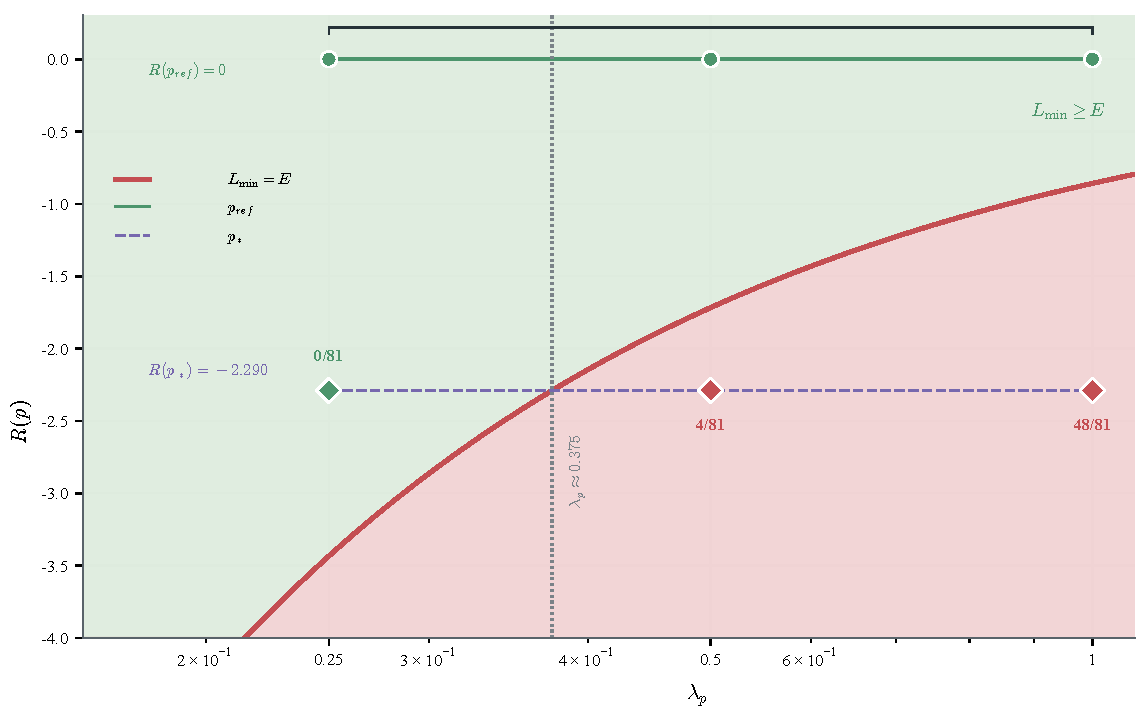
\includegraphics[width=0.90\linewidth]{images/no2/P2R_F09_配比接口物理门槛.pdf}
\caption{配比迁移强度与配比响应共同决定的物理可行域}
\label{fig:p2_mixture_gate}
\end{figure}

图~\ref{fig:p2_mixture_gate} 以 $\min\widehat L=E$ 为边界将情景空间分为物理可行区和阻断区。参考配比满足 $R(\boldsymbol p_{\mathrm{ref}})=0$，在已检查强度范围内始终不跌破不可约损失；近优配比情景在 $\lambda_0=0.5$ 和 $1$ 时分别有 $4/81$ 和 $48/81$ 个网格点违规。图中 $\lambda_0\approx0.375$ 是当前模型情景下的解析门槛，而非由跨体系共同实验识别得到的经验常数。

上述结果说明当前非零配比迁移情景可能进入基础标度律不支持的预测区域。因此，中心标度律模型和固定配比接口通过验收，而联合配比接口暂不具备决策使用条件。后续资源配置分析仅采用 $\boldsymbol p=\boldsymbol p_{\mathrm{ref}}$、$\lambda_0=0$ 的主接口。

综合模型选择、质量分块验证和配比物理门槛检查，本问形成表~\ref{tab:p2_interface} 所示的分层输出；第~\ref{sec:problem3} 节只在 $\boldsymbol p=\boldsymbol p_{\mathrm{ref}}$、$\lambda_0=0$ 下优化 $N$、$D$ 和 $Q_A$。

\begin{table}[!htbp]
\centering
\small
\setlength{\tabcolsep}{4pt}
\caption{问题二向问题三传递的冻结接口}
\label{tab:p2_interface}
\begin{tabular}{p{0.25\linewidth}p{0.34\linewidth}p{0.31\linewidth}}
\toprule
接口 & 冻结内容 & 决策状态 \\
\midrule
基础标度律 & $E,A,B,\alpha,\beta$ 及 $n=N/10^9,d=D/10^9$ & 通过，进入问题三 \\
质量修正 & GQ2 的 $c_Q,\nu_Q$ 与 $Q_{\mathrm{eff}}=h_{s_Q}(Q_A)$ & 通过，$s_Q$ 作情景参数 \\
参考锚点 & $Q_{\mathrm{ref}}=0.5389559588$，$\boldsymbol p=\boldsymbol p_{\mathrm{ref}}$ & 通过，作为中心情景 \\
配比迁移 & $\lambda_0(n/n_0)^{\delta_p}R(\boldsymbol p)$ & 未通过，仅作敏感性分析 \\
支持域标记 & B1/B7 观测域、单分量外推和桥接缺口 & 随问题三每个方案一并传递 \\
\bottomrule
\end{tabular}
\end{table}

\subsubsection{外部验证、稳健性与适用边界}

图~\ref{fig:p2_external_validation} 汇总冻结经典标度律的跨来源预测。B2、B4 和 B5 分别代表半合成族外轨迹、跨模型族记录和公开文献数据；B10 的 Loss 来源于估算结果，因此只作量级对照，不增加独立观测证据。

\begin{center}
\centering
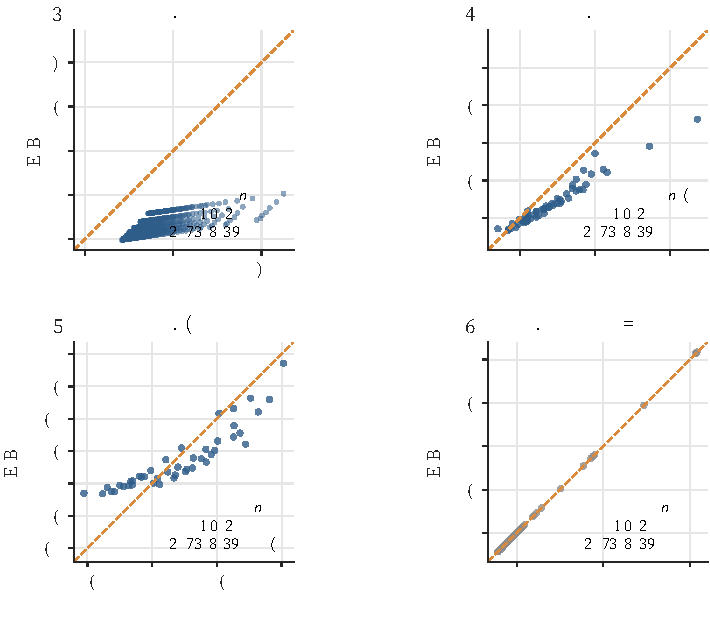
\includegraphics[width=0.66\linewidth]{images/no2/P2R_F10_经典标度律外部证据验证.pdf}
\captionof{figure}{冻结经典标度律的跨来源预测诊断}
\label{fig:p2_external_validation}
\end{center}

图~\ref{fig:p2_external_validation} 中，B2 的 RMSE 为 $1.243085$，存在明显绝对偏差；B4 与 B5 的 Spearman 相关系数分别为 $0.982982$ 和 $0.958808$；B10 虽接近 $1{:}1$ 线，但属于估算值。因此，跨来源分析只检验组内趋势和排序，不直接比较绝对 Loss。

剔除 B1 中 $D<2$（十亿 Token）的 $32$ 个早期检查点后，参数最大相对变化仅为 $0.052965\%$，表明估计稳定。B9 仅界定外推边界，B10 不能替代真实大模型训练验证；因此，超出 B1/B7 支持域的预测均保留外推标记，并结合验证证据谨慎解释。
